\documentclass{standalone}

\usepackage{ tikz }
\usetikzlibrary{automata, positioning, arrows}

\begin{document}
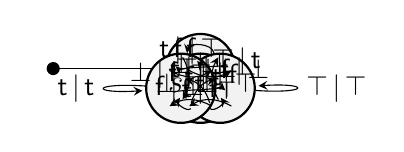
\begin{tikzpicture}[
        ->,
        >=stealth,
        node distance=0.25cm,
        every state/.style={font=\large, thick, fill=gray!10},
        initial text=$ $,
        initial distance=1.5cm,
        every initial by arrow/.style={*->},
        every edge/.append style={},
        yscale=-1,
        x=20pt,
        y=20pt
    ]
    \node[state, initial] (bot) {\(s_\bot\)};
    \node[state, below of=bot] (f) {\(s_\mathsf{f}\)};
    \node[state, right of=f] (top) {\(s_\top\)};
    \node[state, left of=f] (t) {\(s_\mathsf{t}\)};

    \draw (bot) edge[bend right, pos=0.25, above] node{\( \mathsf{t} \,|\, \bot\)} (t)
    (bot) edge[bend right, pos=0.25, left] node {\( \mathsf{f} \,|\, \bot\)} (f)
    (bot) edge[bend left, pos=0.25, above] node{\( \top \,|\, \bot\)} (top)
    (bot) edge[loop above] node{\( \bot \,|\, \bot\)} (bot)
    (t) edge[loop left] node{\( \mathsf{t} \,|\, \mathsf{t}\)} (t)
    (t) edge[bend left, pos=0.2, above] node{\( \mathsf{f} \,|\, \mathsf{t}\)} (f)
    (t) edge[bend left=80, pos=0.25, above left] node{\( \bot \,|\, \mathsf{t}\)} (bot)
    (t) edge[bend right=50, pos=0.2, right] node{\( \top \,|\, \mathsf{t}\)} (top)
    (f) edge[loop below] node{\( \mathsf{f} \,|\, \mathsf{f}\)} (f)
    (f) edge[bend left, pos=0.4, above] node{\( \top \,|\, \mathsf{f}\)} (top)
    (f) edge[bend left, pos=0.2, above] node{\( \mathsf{t} \,|\, \mathsf{f}\)} (t)
    (f) edge[bend right, pos=0.4, left] node{\( \bot \,|\, \mathsf{f}\)} (bot)
    (top) edge[loop right] node{\( \top \,|\, \top\)} (top)
    (top) edge[bend left=80, pos=0.2, below right] node{\( \mathsf{f} \,|\, \bot\)} (t)
    (top) edge[bend left, pos=0.2, above] node{\( \mathsf{f} \,|\, \top\)} (f)
    (top) edge[bend right=80, pos=0.25, above right] node{\( \bot \,|\, \top\)} (bot)
    ;
\end{tikzpicture}
\end{document}